\subsection{Quality Evaluation Across Aggregate Functions}
\label{sec:results_flights}
%
In these experiments we evaluated the quality of the recommended visualizations produced by our proposed techniques 
 across different aggregate functions, namely: \texttt{count, sum, avg, min, max}. 
%
The dataset used is the Flights database with 10 dimension attributes and 10 measures attributes. 
%
We run these experiments to assess the quality of the recommended views over each aggregate function separately with a view space size $SP = 1 \times 10 \times 10 = 100$ possible views.
%
 A utility of a view is measured using the Earth Movers Distance (EMD).
%All Experiments were executed  5 times and obtained the averaged results, we concerned with evaluating the 

We report the accuracy and distance error of views produced by our proposed algorithms by varying the 
limited number of views $R$ while $K = 20$. 
%
In these experiments, we use the following query as our target view:
%
\begin{center}
\texttt{$Q:$ SELECT * FROM Flights WHERE uniquecarrier ='American Airlines Inc.' }
\end{center}
%

%In the next experiments, we vary $R$ � the number of limited visualizations that explored denoted as \emph{Views Limit} 
%to recommend $K=20$ visualizations and measure the accuracy, and error-distance for each of our
%strategies along different aggregate functions.\\

In summary, Sela and DimsHisto algorithms both produce results with accuracy $ > \%80$ for all aggregate functions, especially when $R = 60$, as shown in Figures \ref{fig:SumA2},\ref{fig:AvgA2}, and \ref{fig:CountA2}. 
%
Moreover, they produce results with $\%100$ accuracy when $R > 60 $. 
%
$Sela$ does slightly better than $DimsHisto$ in terms of accuracy, as $Sela$ evaluates the recommended views by capturing the change of the selectivity ratios of dimension attributes that create views in both result set and reference set. 
%
However, $DimsHisto$ scores $\%100$  accuracy in Figure \ref{fig:CountA2} for aggregate function \texttt{count} because the generated histograms from this algorithm are similar to the views created by counting dimension attribute values across different measure attributes. 
%
Algorithm $Diff_DVal$ has the lowest accuracy and the highest distance error among the other algorithms specially for aggregate functions \texttt{max, min} as shown in Figures \ref{fig:MaxA2} and \ref{fig:MinA2} as it assess recommended views based on the difference of the distinct values only. 
%
\begin{figure}[t]
  \begin{subfigure}[b]{0.32\textwidth}
    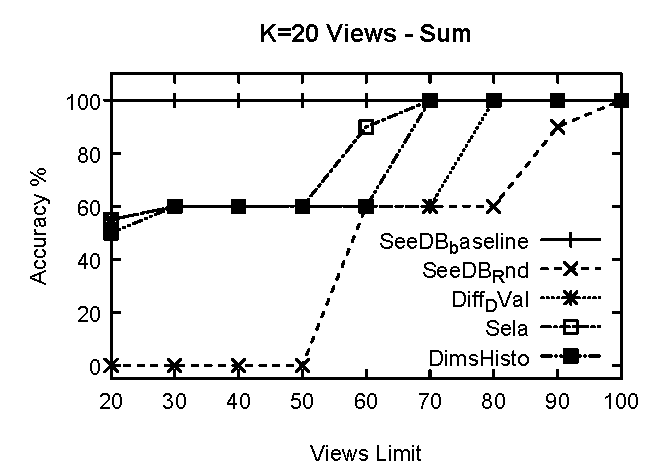
\includegraphics[width=\textwidth]{SumA2.pdf}
    \caption{ \texttt{sum} }
     \label{fig:SumA2}%
  \end{subfigure}
  %
  \begin{subfigure}[b]{0.32\textwidth}
    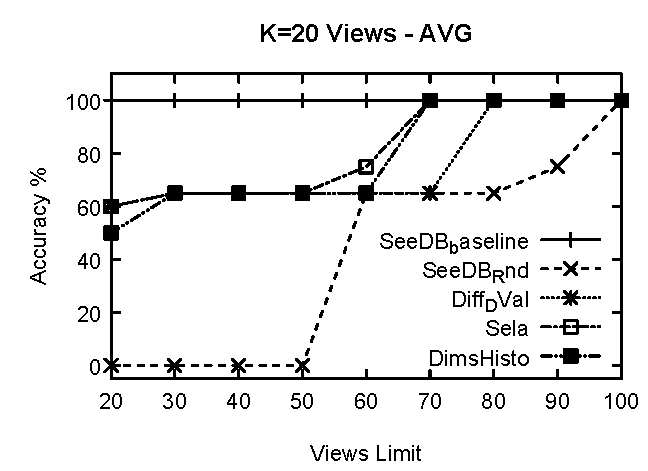
\includegraphics[width=\textwidth]{AvgA2.pdf}
     \caption{ \texttt{avg}}
        \label{fig:AvgA2}
  \end{subfigure}
  \begin{subfigure}[b]{0.32\textwidth}
    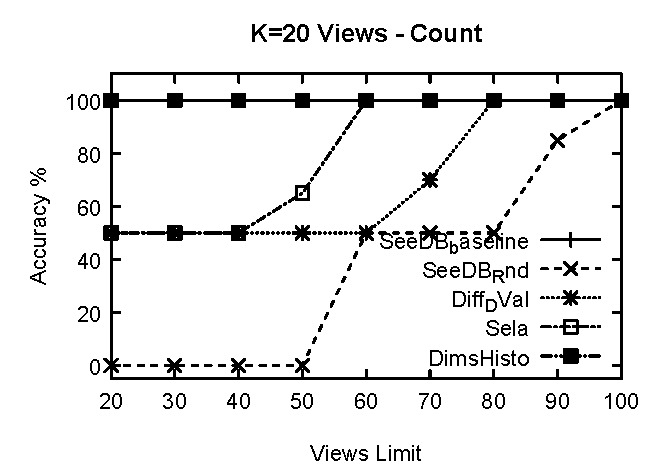
\includegraphics[width=\textwidth]{CountA2.pdf}
     \caption{ \texttt{count}}
        \label{fig:CountA2}
  \end{subfigure}
  \caption{Accuracy on varying view space $R$ and $K = 20$}
\end{figure}

\begin{figure}[t]
  \begin{subfigure}[b]{0.32\textwidth}
    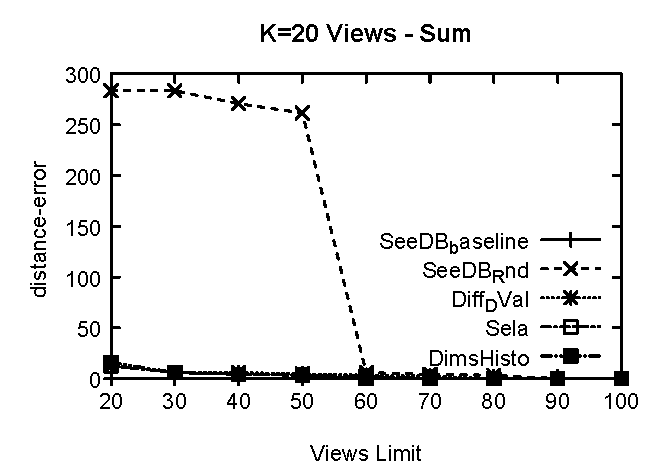
\includegraphics[width=\textwidth]{SumD2.pdf}
    \caption{ \texttt{sum}}
        \label{fig:SumD2}%
  \end{subfigure}
  %
  \begin{subfigure}[b]{0.32\textwidth}
    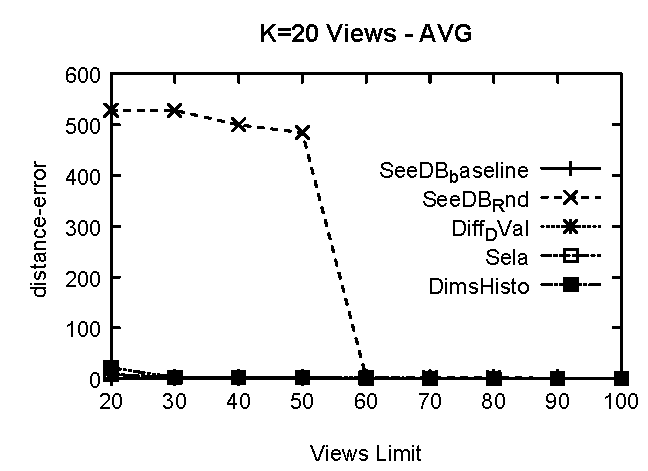
\includegraphics[width=\textwidth]{AvgD2.pdf}
     \caption{ \texttt{avg}}
        \label{fig:AvgD2}
  \end{subfigure}
  \begin{subfigure}[b]{0.32\textwidth}
    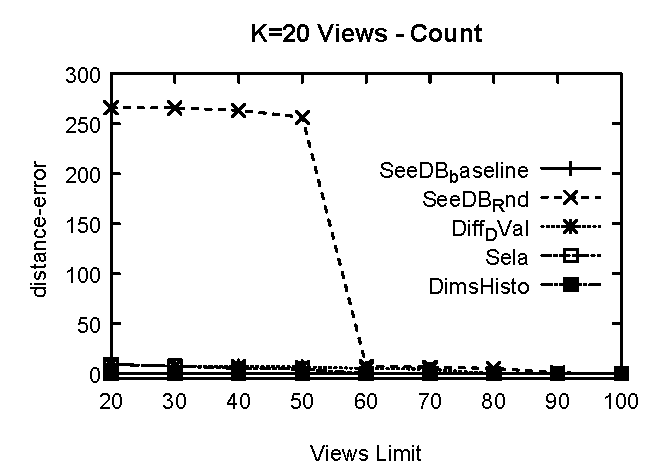
\includegraphics[width=\textwidth]{CountD2.pdf}
     \caption{ \texttt{count}}
        \label{fig:CountD2}
  \end{subfigure}
  \caption{Distance error on varying view space $R$ and $K = 20$}
\end{figure}

As shown in Figures \ref{fig:SumD2},\ref{fig:AvgD2} and \ref{fig:CountD2}, the proposed algorithms produce results near-zero distance-error for all aggregate functions compared with lower baseline strategy $SeeDB_Rnd$ which produce views with low quality however, the quality of the recommended views produced by the proposed algorithms is almost near to the same utilities of views output by the top baseline $SeeDB baseline$. 
%
The distance-error of results in the first view limits=20 and 30 views as shown in Figures \ref{fig:MaxD2} and \ref{fig:MinD2} is high specially for the aggregate function \texttt{min} because functions such as \texttt{min, max} are not docile for sampling but the proposed algorithms still score very low distance-error.
 
 %\begin{center}
  \begin{figure}[t]
  \centering
  \begin{subfigure}[b]{0.42\textwidth}
    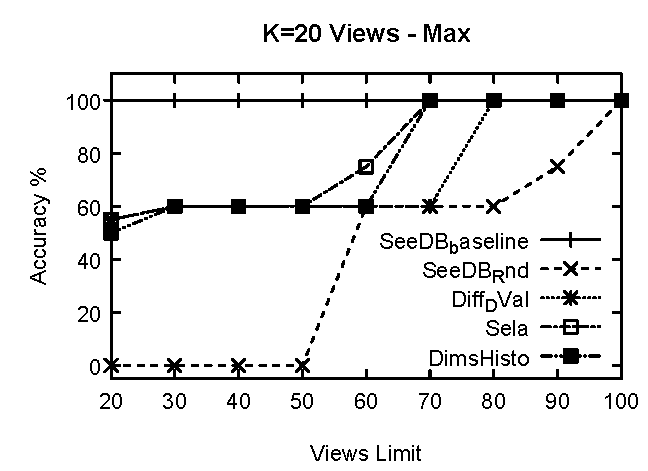
\includegraphics[width=\textwidth]{MaxA2.pdf}
    \caption{ \texttt{max}}
        \label{fig:MaxA2}%
  \end{subfigure}
  %
  \begin{subfigure}[b]{0.42\textwidth}
    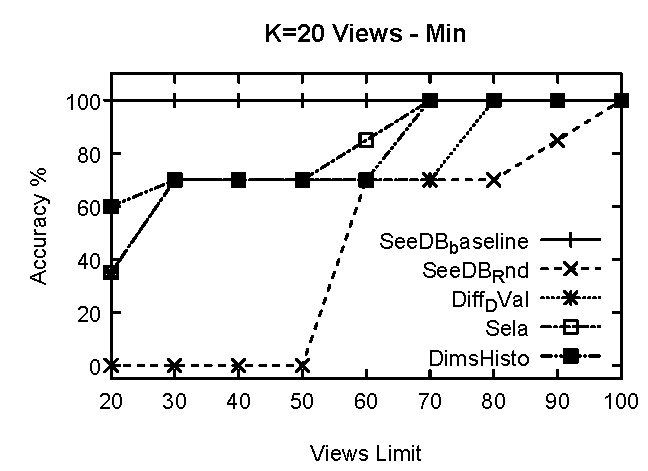
\includegraphics[width=\textwidth]{MinA2.pdf}
     \caption{ \texttt{min}}
        \label{fig:MinA2}
	% \caption{Accuracy on varying view space sizes for the Algorithms $Sela$ ,$Diff_DVal$, $DimsHisto$, and $SeeDB_Rnd$}
  \end{subfigure}
  \caption{Accuracy on varying view space $R$ and $K = 20$}
\end{figure}
%\end{center}

%\begin{center}
  
\begin{figure}[t]
  \centering

  \begin{subfigure}[b]{0.42\textwidth}
    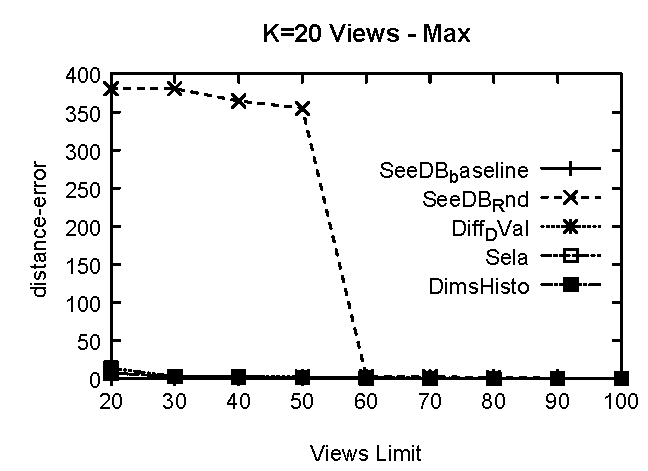
\includegraphics[width=\textwidth]{MaxD2.pdf}
    \caption{ \texttt{max}}
        \label{fig:MaxD2}%
  \end{subfigure}
  %
  \begin{subfigure}[b]{0.42\textwidth}
    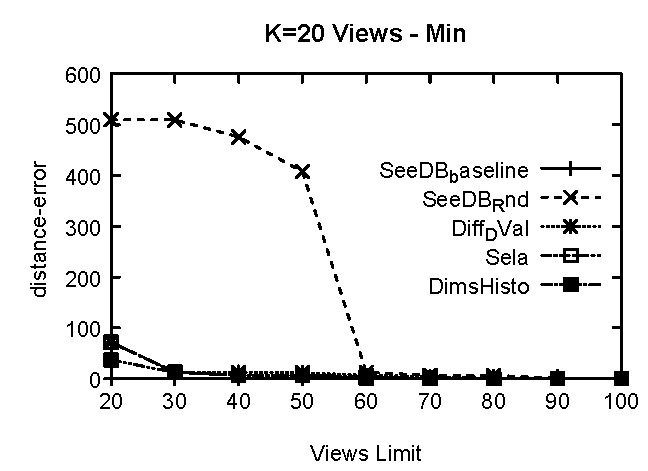
\includegraphics[width=\textwidth]{MinD2.pdf}
     \caption{ \texttt{min}}
        \label{fig:MinD2}
  \end{subfigure}
  
  \caption{Distance error on varying view space $R$ and $K = 20$}
\end{figure}

%\end{center}

The proposed techniques recommend high quality views in different views limits. 
%
Furthermore, the accuracy is increasing without fluctuating along various views limits $R$ and similarly the distance-error is declining while increasing the number of explored views $R$. 
%
In the worst cases, the accuracy and the distance-error remain constant while increasing the number of explored views $R$.% but they don't decrease. \\
%%%%%%%% Second Expr

In the following experiments, we vary $K$ and fix the number of explored visualizations as $R = 70$ and measure the accuracy, and error-distance for each of our
strategies along different aggregate functions. 
%
We pay special attention to $K = 10$ and $K = 20$ because empirically these $K$ values are used most commonly.
%
As the Figures \ref{fig:SumA1}, \ref{fig:AvgA1}, \ref{fig:CountA1}, \ref{fig:MaxA1} and\ref{fig:MinA1} show,  $Sela$ and $DimsHisto$ algorithms both produce results with accuracy $\%100$ and zero distance-error when $K = 10$ and $K = 20$ for all aggregate functions.
%
Moreover, $Diff_DVal$ algorithm scored accuracy $\%100$ in the first number of recommended views $K = 10$. 
%
Although, $Diff_DVal$ obtains the same accuracy as $SeeDB_Rnd$ for all aggregate functions, the $Diff_DVal$ scores much better distance-error than $SeeDB_Rnd$, as shown in Figures \ref{fig:SumD1}, \ref{fig:AvgD1}, \ref{fig:CountD1}, \ref{fig:MaxD1} and\ref{fig:MinD1}. 
%
As discussed in the previous experiment, the $DimsHisto$ algorithm scores accuracy $\%100$ specifically when the aggregate function is \texttt{count}. 
%
It also succeeds to recommend views with $\%100$ accuracy and zero distance-error for aggregate functions \texttt{count, sum, avg} as shown in Figures \ref{fig:SumA1}, \ref{fig:AvgA1} and \ref{fig:CountA1}. 
%
In addition, we found that $Sela$ and $DimsHisto$ algorithms produce high quality views with $\%100$ accuracy and zero distance-error for \texttt{max} aggregate function. 
%
Also, they obtain $ > \%75$ and $ < 0.2$ distance error for \texttt{min} aggregate function when $K = 70$ as shown in Figures \ref{fig:MaxD1} and \ref{fig:MinD1}, respectively.

\begin{figure}[t]
  \begin{subfigure}[b]{0.32\textwidth}
    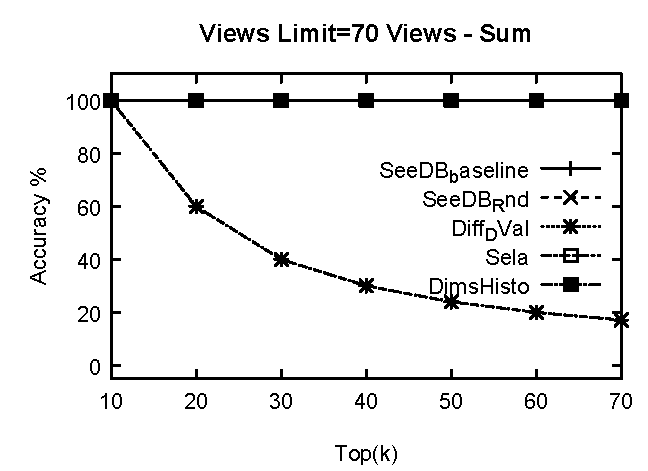
\includegraphics[width=\textwidth]{SumA1.pdf}
    \caption{ \texttt{sum}   }
        \label{fig:SumA1}%
  \end{subfigure}
  %
  \begin{subfigure}[b]{0.32\textwidth}
    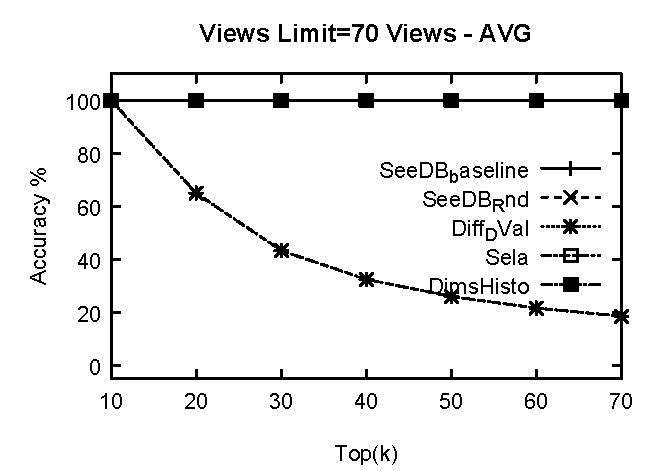
\includegraphics[width=\textwidth]{AvgA1.pdf}
     \caption{ \texttt{avg} }
        \label{fig:AvgA1}
  \end{subfigure}
  \begin{subfigure}[b]{0.32\textwidth}
    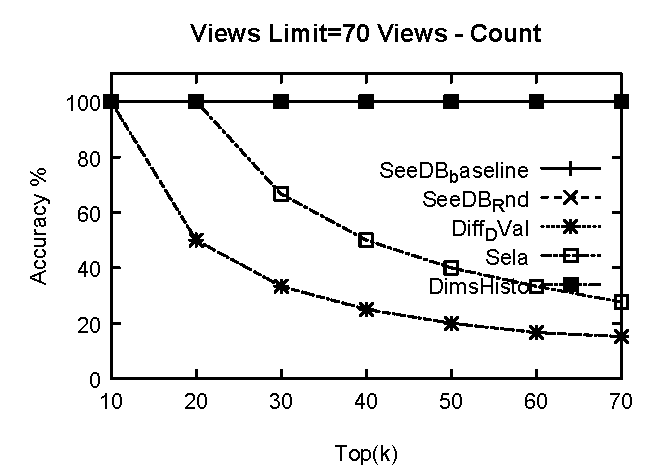
\includegraphics[width=\textwidth]{CountA1.pdf}
     \caption{ \texttt{count}  }
        \label{fig:CountA1}
  \end{subfigure}
  \caption{Accuracy while varying $K$ and $R = 70$}
\end{figure}

As Figures \ref{fig:SumD1}, \ref{fig:AvgD1}, \ref{fig:CountD1}, \ref{fig:MaxD1} and\ref{fig:MinD1} show, the $Diff_DVal$ approach scores the same accuracy produced by $SeeDB_Rnd$ and obtains very low distance error along all aggregate functions when compared with $SeeDB_Rnd$.
%
Hence, our proposed approaches boost the accuracy of the recommended views for the mostly common used $K$ values. 
%
Moreover, the $Sela$ and $DimsHisto$ algorithms achieve better quality results than $Diff_DVal$ because they capture the data distribution in the dimension attributes by using selectivity ratios and frequency histograms.
 
\begin{figure}[t]
  \begin{subfigure}[b]{0.32\textwidth}
    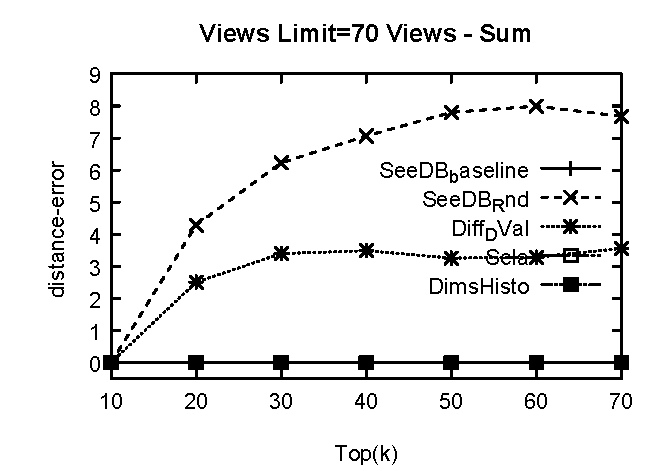
\includegraphics[width=\textwidth]{SumD1.pdf}
    \caption{ \texttt{sum}   }
        \label{fig:SumD1}%
  \end{subfigure}
  %
  \begin{subfigure}[b]{0.32\textwidth}
    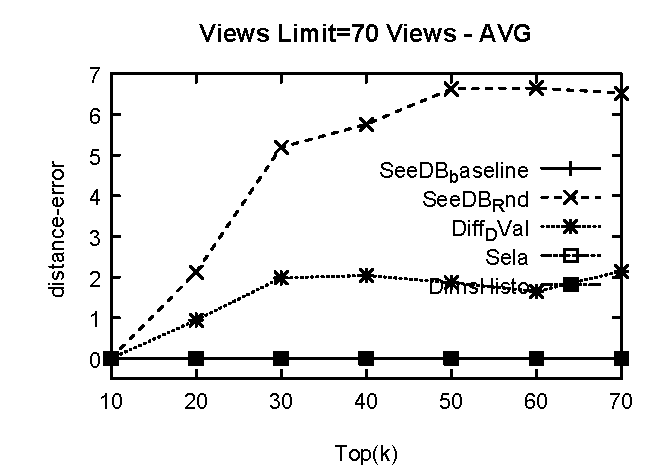
\includegraphics[width=\textwidth]{AvgD1.pdf}
     \caption{ \texttt{avg} }
        \label{fig:AvgD1}
  \end{subfigure}
  \begin{subfigure}[b]{0.32\textwidth}
    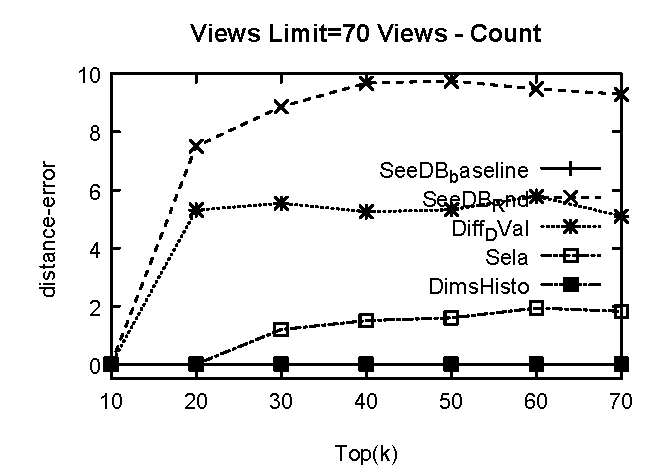
\includegraphics[width=\textwidth]{CountD1.pdf}
     \caption{ \texttt{count} }
        \label{fig:CountD1}
  \end{subfigure}
  \caption{Distance error on varying $K$ and $R = 70$}
\end{figure}


 % \begin{center}
    
  \begin{figure}[t]
  \centering
%\end{figure}
  \begin{subfigure}[b]{0.42\textwidth}
    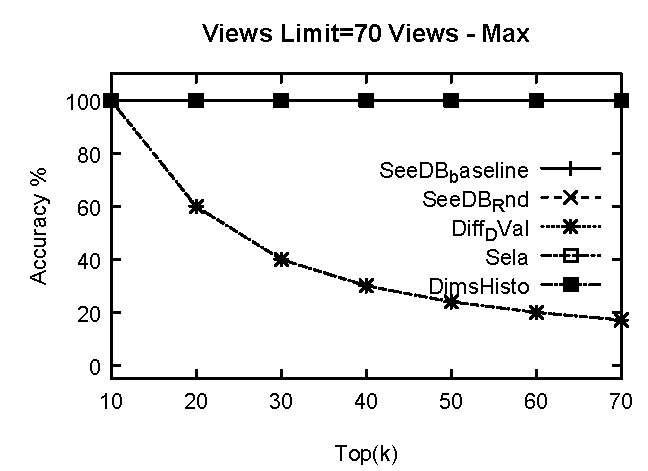
\includegraphics[width=\textwidth]{MaxA1.pdf}
    \caption{ \texttt{max}   }
        \label{fig:MaxA1}%
  \end{subfigure}
  %
  \begin{subfigure}[b]{0.42\textwidth}
    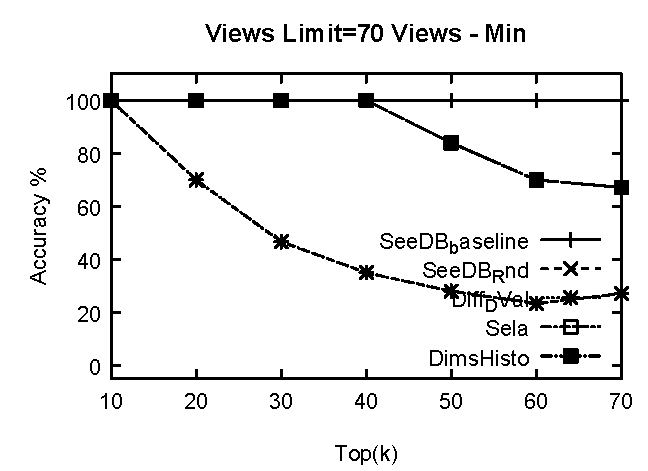
\includegraphics[width=\textwidth]{MinA1.pdf}
     \caption{ \texttt{min}  }
        \label{fig:MinA1}
  \end{subfigure}
  
  \caption{Accuracy on varying $K$ and $R = 70$}
\end{figure}
%\end{center}

%\begin{center}
  
\begin{figure}[t]
  \centering
  \begin{subfigure}[b]{0.42\textwidth}
    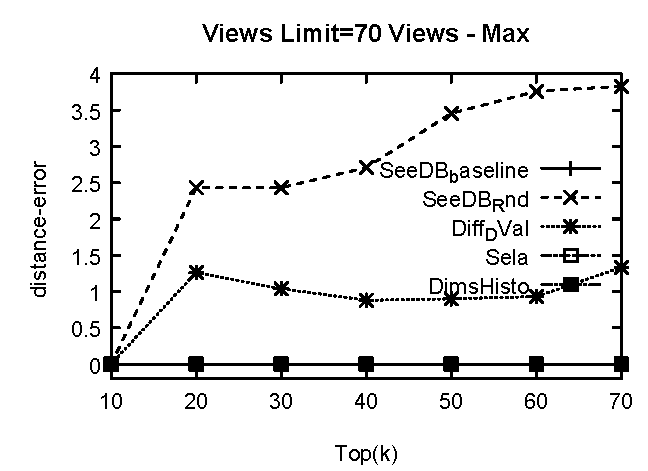
\includegraphics[width=\textwidth]{MaxD1.pdf}
    \caption{ \texttt{max}   }
        \label{fig:MaxD1}%
  \end{subfigure}
  %
  \begin{subfigure}[b]{0.42\textwidth}
    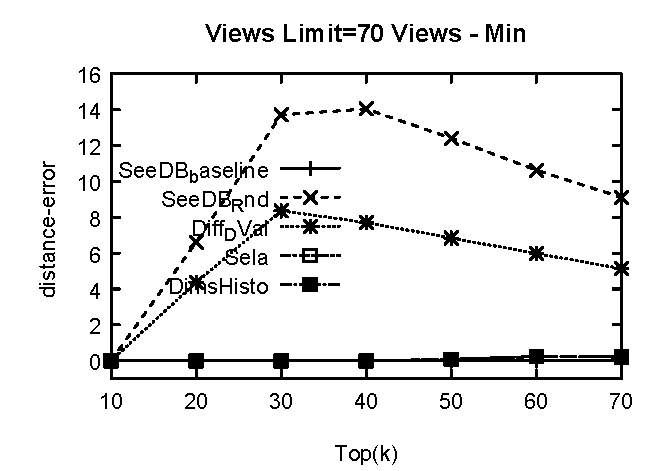
\includegraphics[width=\textwidth]{MinD1.pdf}
     \caption{ \texttt{min}}
        \label{fig:MinD1}
  \end{subfigure}
  
  \caption{Distance error on varying $K$ and $R = 70$}
\end{figure}